\documentclass[main.tex]{subfiles}

\begin{document}

  \section{Computational aspects}

   \subsection{Complexity analysis}

   We recall the parameters of the problem: we consider a superelliptic curve $\cu$ given by
   $\caff:y^m=f(x)$ with $f \in \C[x]$ separable of degree $n$. The genus $g$ of $\cu$ satisfies
   $$g \leq \frac{(m-1)(n-1)}2=O(mn).$$

   Let $D$ be some desired accuracy (a number of digits). The computation of
   the Abel-Jacobi map on $\cu$ has been decomposed into the
   following list of tasks:
   \begin{enumerate}
       \item computing the $(n-1)$ vectors of elementary integrals,
       \item computing the big period matrix $\Omega=(\OA,\OB)$ \eqref{m-eq:OAOB},
       \item computing the small period matrix $\tau = \OA^{-1}\OB$ \eqref{m-eq:tau},
       \item evaluating the Abel-Jacobi map at a point $P \in \cu$,
   \end{enumerate}
   all of these to absolute precision $D$.

   Let $N(D)$ be the number of points of numerical integration.
   If $m=2$, we have
   $N(D)=O(D)$ using Gauss-Chebychev integration, while $N(D)=O(D\log D)$
   via double exponential integration.

   For multiprecision numbers, we consider (see \cite{BrentZimmermann}) that the multiplication has
   complexity $\cmul(D)=O(D \log^{1+\varepsilon}D)$,
   while simple transcendental functions (log, exp, tanh, sinh,\dots) can be evaluated
   in complexity $\ctrig(D)=O(D\log^{2+\varepsilon} D$).
    Moreover, we assume that inversion and multiplication of a $g \times g$ matrix can be done using
    $O(g^{\eta})$ multiplications for some constant $2 < \eta < 3$.
   
   \subsubsection{Computation of elementary integrals}

   For each elementary cycle $\gamma_e\in \Gamma$, we evaluate numerically the vector of $g$
   elementary integrals from \eqref{eq:elem_num_int} as sums of the form
   \begin{equation}
       I_{a,b} \approx \sum_{k=1}^N w_k\frac{u_k^{i-1}}{y_k^j}
   \end{equation}
   where $N$ is the number of integration points, $w_k,u_k$ are integration weights and points,
   and $y_k=\ytab(u_k)$.

   We proceed as follows:
   \begin{itemize}
   \item for each $k$, we evaluate the absissa and weight $u_k,w_k$ using
       a few \footnote{this can be reduced to evaluating only one exponential
       and a few multiplications.} trigonometric or hyperbolic functions,
   \item we compute $y_k=\ytab(u_k)$ using $n-2$ multiplications and one $m$-th root,
       as shown in \S \ref{m-subsec:computing_roots} below;
   \item starting from $w_k\frac{1}{y_k}$, we evaluate all $g$ terms $w_k\frac{x_k^{i-1}}{y_k^j}$
       each time either multiplying by $u_k$ or by $\frac{1}{y_k}$, and add each to the corresponding
       integral.
   \end{itemize}

   Altogether, the computation of one vector of elementary integrals takes
   \begin{equation}\label{eq:elem_int_complexity}
    \ctot(D) := N(D)\ctrig(D)+N(D)(n-1)\cmul(D)+N(D)g\cmul(D)
   \end{equation}
    operations,
   so that depending on the integration scheme we obtain:
   \begin{thm}\label{thm:complexity_integrals}
       Each of the $(n-1)$ elementary vector integrals can be computed to precision $D$ using
       \begin{equation}
           O(N(D)\cmul(D)(g+\log D)) =
           \begin{cases}
               O(D^2\log^{1+\varepsilon} D (g + \log D)) \text{ operations, if $m=2$,}\\
               O(D^2\log^{2+\varepsilon} D (g + \log D)) \text{ operations, if $m>2$.}
           \end{cases}
       \end{equation}
   \end{thm}
   %\begin{proof}
   %  Plugging in $N(D),T(D),M(D)$ in equation \eqref{m-eq:elem_int_complexity} and using that $n-1 = O(g)$.
   %\end{proof}

   \subsubsection{Big period matrix}

   One of the nice aspects of the method is that we never compute
   the dense matrix $\OC\in\C^{g\times 2g}$ from \eqref{m-eq:OC}, but
   keep the decomposition of periods in terms of the elementary integrals
   $\int_{\gamma_e}\omega_{i,j}$ in $\C^{g\times (n-1)}$.

   Using the symplectic base change matrix $S$ introduced
   in \S~\ref{m-subsec:symp_basis}, the homology basis is given
   by equations of the form
   \begin{equation}
       \label{eq:base_change_cycles}
       \alpha_i = \sum_{e,l} s_{e,l}\gamma_e^{(l)}
   \end{equation}
   where $\gamma_e,e\in E$ spans the elementary cycles
   and $l\in\Z/m\Z$ their shifts,
   and $s_{e,l}\in\Z$ are coefficients of the matrix $S$. 

   We use \eqref{m-eq:periods} to compute the coefficients of the big period
   matrix $(\OA,\OB)$, so that each term of \eqref{m-eq:base_change_cycles}
   involves only a fixed number of multiplications.

   In practice, these sums are sparse and their coefficients are very small integers
   (less than $m$), so that the change of basis is performed using
   $O(g^2D\log^{1+\varepsilon}D)$ operations
   (each of the $O(g^2)$ periods is a linear combination of $O(1)$ elementary integrals,
   the coefficients involving precision $D$ roots of unity).

   However we have no proof of this fact and in general the symplectic reduction
   could produce dense base change with coefficients of size $O(g)$,
   so that we state the far from optimal result
   \begin{thm}
       Given the $(n-1)\times g$ elementary integrals to precision $D$,
       we compute the big period matrix using $O(g^3(D+g)\log(D+g))$ operations.
   \end{thm}

   \subsubsection{Small period matrix}

   Finally, the small period matrix is obtained as $\tau=\OA^{-1}\OB$,
   i.e. one $g\times g$ matrix inversion and one multiplication, which
   can be done using $O(g^{\eta})$ multiplications.
   
   \subsubsection{Abel-Jacobi map}
   
  This part of the complexity analysis is based on the results of Section \ref{m-sec:comp_ajm} and assumes that we already computed a big period matrix and all related data.
   
  Let $\ctot(D)$ be the number of operations needed to compute a vector of $g$ elemenatary integrals  (see \eqref{m-eq:elem_int_complexity}). The complexity class of $E(D)$ in $O$-notation is given in
  Theorem \ref{m-thm:complexity_integrals}.
  
   \begin{thm} \
   \begin{itemize}
     \item[(i)] For each finite point $P \in \caff$ we can compute $\int_{P_0}^P \bar\w$ to precision $D$ using 
      $\ctot(D)$ operations. 
     \item[(ii)] For each infinite point $P_{\infty} \in \cu$ we can compute $\int_{P_0}^{P_{\infty}} \bar\w$ to precision $D$ using
      \begin{itemize}
       \item[$\bullet$] $n$ vector additions in $\C^g$, if $\delta = \gcd(m,n) = 1$,
       \item[$\bullet$] $n \ctot(D)$ operations in the case of Theorem \ref{m-thm:ajm_inf_ord1},
       \item[$\bullet$] $n(n+\frac{m}\delta)\ctot(D)$ operations  in the case of Theorem \ref{m-thm:ajm_inf_ordgt1}.
      \end{itemize}
      \item[(iii)] Reducing a vector $v \in \C^g$ modulo $\Lambda$ can be done using $O(g^{\eta})$ multiplications.
    \end{itemize}
  \end{thm}
   \begin{proof}
    \begin{itemize}
     \item[(i)] Follows from combining the results from \S \ref{m-subsec:ajm_ram_pts} and Remark \ref{m-rmk:ajm_finite_int}.
     \item[(ii)] The statements follow immediately from \S \ref{m-subsec:ajm_inf_cop}, Theorem \ref{m-thm:ajm_inf_ord1} and Theorem \ref{m-thm:ajm_inf_ordgt1}.
     \item[(iii)] By \S \ref{m-subsec:lat_red}, the reduction modulo the period lattice requires one $2g \times 2g$ matrix inversion and one multiplication.
    \end{itemize}
   \end{proof}

   \subsection{Integration parameters}

   \subsubsection{Gauss-Chebychev case}

   We have a parametrization
   $ε_r = \set{ \cosh(r+it) = \cos(t-ir), t\in]-π,π] }$
   of the ellipse.

   \begin{figure}[H]
       \begin{center}
       \includegraphics[width=5cm,page=3]{images/ellipse.pdf}
   \end{center} \caption{Ellipse parameters.}
   \label{fig:ellipse}
   \end{figure}

   The sum of its semi-axes is $e^{r}$
   and one needs 
   \[
       N \geq \frac{D+\log(2πM(r)+e^{-D})}{2r}
   \]
   to have $\abs{E(N)}\leq e^{-D}$.

   The distance $d_k=\dist(u_k,ε_r)$ from a branch point $u_k$
   to the ellipse $ε_r$ can be computed
   applying Newton method to the scalar product function
   $f(t) = \Re(\overline{z'}(u_k-z))$, where $z = \cos(t-ir)$ and
   we take $t=\Re(\arccos(u_k))$ as a starting point.
   By convexity of the ellipse,
   the solution is unique on the quadrant containing $u_k$.

   \subsubsection{Choice of $r$}
   
   Let $\abs{u_k-1}+\abs{u_k+1}=2\cosh(r_k)$. We need to choose
   $r<r_0=\min_k r_k$ (so that $u_k\not\in ε_r$) in order to minimize
   the number of integration points \eqref{eq:Ngc}. We first
   estimate how the bound $M(r)$ varies for $r<r_0$.
   \begin{itemize}
       \item 
   For all $k$ such that $r_k > r_0$, we compute
   explicitly the distance $d_k=\dist(u_k,ε_{r_0})<\dist(u_k,ε_r)$.
   \item
   For $k$ such that $r_k=r_0$, we use first order approximation
   \[ \dist(u_k,Z_{r-η}) = η D_k + O(η^2) \]
   where $D_k = \abs{\frac{\partial u_k}{\partial r_k}} = \abs{\sin(t_k-ir_k)}$.
   \end{itemize}

   Let $K$ be the number of branch points $u_k$ such that $r_k=r_0$ and 
   \[ M_0 = \sqrt{\prod_{r_k = r_0} D_k\prod_{r_k>r_0}d_k}^{-1}, \]
   then the integrand is bounded on $ε_{r_0-η}$ by
   \[ M(r_0-η) = M_0 \sqrt{η}^{-K} (1+O(η)). \]
   Plugging this into \eqref{eq:Ngc}, the number of integration points
   satisfies
   \[
       2N = \frac{D+\log(2πM_0) - K/2 \log(η) }{r_0-η}(1+O(η)).
   \]

   The main term is minimized for $η$ satisfying
   $η(2\frac{D+\log(2πM_0)}K+1-\log(η))=r_0$. The solution
   can be written as a Lambert function or we use
   the approximation
   \[ r = r_0 - η = r_0 ( 1 - \frac{1}{A+\log\frac{A}{r_0}}), \]
   where $A = 1+\frac2K(D+\log(2πM_0))$.
 
   \subsubsection{Double-exponential case}

   We use the parametrization
   $\partial Z_r = \set{ z = \tanh(λ\sinh(t+ir), t\in\R }$ to compute
   the distance from a branch point $u_k$ to $Z_r$ by Newton method
   as before.
   %$f(t) = \Re(\overline{z'}(u_k-z))$, where $z = \tanh(λ\sinh(t+ir))$
   %and starting point $t=\Re(z^{-1}(p))$.

   Unfortunately the solution may not be unique, so once
   the parameter $r<r_0$ is chosen (see below), we use ball arithmetic to compute a rigorous
   bound of the integrand on the boundary of $Z_r$. The process consists in
   recursively subdividing the interval until the images of the subintervals by the
   integrand form an $ε$-covering.

   \paragraph{Choice of $r$}

   We adapt the method used for Gauss-Chebychev. This time the number $N$ of integration
   points is obtained from equation \eqref{eq:de-parameters}.
   
   Writing $u_k = \tanh(λ\sinh(t_k+ir_k))$, we must choose
   $r<r_0=\min_k r_k$ to ensure $u_k\not\in Z_r$. Let 
   \[ M_0 = (\prod_{r_k = r_0} D_k\prod_{r_k>r_0}d_k)^{-j/m} \]
   where $d_k=\dist(u_k,Z_{r_0})<\dist(u_k,Z_r)$ and
   \[ D_k = \abs{\frac{\partial u_k}{\partial r_k}} = \abs{\frac{λ \cosh(t_k+ir_k)}{\cosh(λ\sinh(t_k+ir_k))^2}} \]
   is such that $\dist(u_k,Z_{r-η}) = η D_k + O(η^2)$, then
   the integrand is bounded on $Z_{r_0-η}$ by
   \[ M_2 = M_0 η^{-\frac{jK}m} (1+O(η)). \]
   Then
   \[ h = \frac{2π(r_0-η)}{D+\log(2B(r_0,α)M_0)-jK/m\log(η)}+O(η) \]
   and the maximum is obtained for $η$ solution of $η(A-\log η)=r_0$
   where $A=1+\frac{m}{jK}(D+\log(2B(r_0,α)M_0))$.
 
   \subsection{Implementation tricks}

   Here we simply give some ideas that we used in our implementation(s) to improve constant factors hidden in the big-$O$ notation, i.e. the absolute running time.

   \subsubsection{Improving branch points}

   As we saw in Section \ref{m-sec:numerical_integration}, the number of integration points
   closely depends on the configuration of branch points.

   In practice, when using double-exponential integration, the constant $r$ is usually bigger than $0.5$
   for random points, but we can exhibit bad configurations with $τ\approx 0.1$.
   In this case however, we can perform a change of coordinate by a Moebius transform
   $x\mapsto \frac{ax+b}{cx+d}$ as explained in Remark \ref{rmk:moebius} to redistribute the points more evenly.

   Improving $τ$ from $.1$ to say $.6$ immediately saves a factor $6$ on the running time.

  \subsubsection{Computing products of complex roots}\label{subsec:computing_roots}

  For numerical integration of the integrals in \eqref{m-eq:periods}
  we need to evaluate
  \begin{equation*}
   \ytab(u) = \prod_{u_k\in U^-} \sqrt[m]{u-u_k}\prod_{u_k\in U^+}\sqrt[m]{u_k-u}
  \end{equation*}
  for $u \in [-1,1]$. Instead of computing $(n-2)$ $m$-th roots for each
  integration point, we compute $q(u)\in\frac12\Z$ such that
  \begin{equation*}
   \ytab(u) = \zeta^q \Big( \prod_{u_k\in U^-}(u-u_k) \prod_{u_k\in U^+} (u_k-u) \Big)\mr
  \end{equation*}
 which can be done by tracking
  the winding number of the product while staying away from the branch cut
  of the $m$-th root.
  For complex numbers $z_1,z_2 \in \C$ we can make a diagram of
  $\frac{\sqrt[m]{z_1}\sqrt[m]{z_2}}{\sqrt[m]{z_1z_2}} \in \{ 1, \zeta,
  \zeta^{-1} \}$, depending on the position of $z_1,z_2$ and their product
  $z_1z_2$ in the complex plane, resulting in the following Lemma:

  \begin{lemma}\label{lemma:wind_numb}
  Let $z_1,z_2 \in \C  \setminus  ]\infty,0]$. Then,
  $$\frac{\sqrt[m]{z_1}\sqrt[m]{z_2}}{\sqrt[m]{z_1z_2}} = \begin{cases}
                                                           \zeta, \quad \text{if} \quad \Im(z_1), \Im(z_2) > 0 \quad \text{and} \quad \Im(z_1z_2) < 0 , \\
                                                           \zeta^{-1}, \text{if} \quad \Im(z_1), \Im(z_2) < 0 \quad \text{and} \quad \Im(z_1z_2) > 0 , \\
                                                           1, \quad \text{otherwise}.
                                                         \end{cases}$$
   For $z \in ]\infty,0]$ we use $\sqrt[m]{z} = \zeta^{\frac{1}{2}} \cdot \sqrt[m]{-z}$.
  \end{lemma}
  \begin{proof}
   Follows from the choices for $\sqrt[m]{\cdot}$ and $\zeta$ that were made in \S \ref{m-subsec:roots_branches}.
  \end{proof}
  This Lemma can easily be turned into an algorithm that computes $q(u)$.

   \subsubsection{Doing real multiplications}\label{subsec:real_mult}

   During integration, the main complexity comes from the multiplication by numerator
   $x_k=u_k-\frac{b+a}2$, which is usually done $g-m-1$ times for each of
   the $N$ integration points (more precisely, as we saw in the proof of Proposition \ref{m-prop:holom_diff}, for each power $j$
   we use the powers $0\leq i\leq n_i = \floor{\frac{nj-δ}m}$, with $\sum n_i = g$).

   Without polynomial shift \eqref{eq:polshift}, this numerator should be
   $x_k=u_k+\frac{b+a}{b-a}$. However, $x_k$ is a complex number while $u_k$
   is real, so computing with $u$ saves a factor almost 2 on the running time.

   
   \subsubsection{Maximal spanning tree}
    As explained in \S \ref{m-subsec:cycles_homo} we integrate along the edges of a maximal-flow spanning tree $T = (X,E)$, where the capacity $r_e$ of an edge $e = (a,b) \in E$ is computed as
    \begin{equation}
     r_e =  \min_{c \in X \setminus \{ a,b\}} \begin{cases}
            \frac{|c-a|+|c-b|}{|b-a|}, \text{ if $m=2$,}\\
            | \Im(\sinh^{-1}(\tanh^{-1}(\frac{2c - b -a}{b-a})/\lambda) |, \text{ if $m>2$.}
            \end{cases}
    \end{equation}
    Although this can be done using low precision $D \approx 20$, computing these capacities for all \\ $(n-1)(n-2)/2$ edges of the complete graph leaves us with
    \begin{equation}
     \begin{cases}
     O(n^3 \cmul(D)) \text{ operations, if $m=2$ and}\\
     O(n^3 \ctrig(D)) \text{ operations, if $m>2$}.
    \end{cases}
    \end{equation}
    For large $n$, the computation of these capacities has a noticable impact on the running time. This can be avoided by computing a \emph{minimal spanning tree} that uses the euclidean distance
    between the end points of an edge as capacity, i.e. taking $r_e = |b-a|$ reduces the complexity to $O(n^2 \cmul(D))$.
    
    Given sufficiently many branch points that are randomly distributed in the complex plane, the shortest edges of the complete graph tend to agree with the edges that are well suited for integration.
    Heuristically we find that starting with $n \approx 15$ this approach becomes favourable.
    
    



    
    
   
   
  \subsection{Further ideas} 
    \todo
    
\biblio
\end{document}
